%\documentclass[mathserif]{beamer}
\documentclass[serif, handout]{beamer} % Handout to ignore pause statements
\usepackage{wasysym,graphicx,pgfpages}
\graphicspath{{images/}}   % figures live in images/
\usepackage{amsfonts,amsmath,amsthm, enumerate}
\usepackage{ragged2e}
\usepackage{bbm}
\justifying
\DeclareMathOperator*{\doublesum}{\sum\sum}
\usepackage{beamerthemesplit}
\usepackage{beamerbasetheorems}
\usepackage{beamerthemeshadow}
\usepackage{centernot}
\newtheorem{prop}{Proposition}
\setbeamertemplate{blocks}[rounded]
\setbeamertemplate{items}[ball]

\usetheme{Frankfurt}
\definecolor{Green}{rgb}{0,0.59,0}
% predefine colors: red, green, cyan, magenta, yellow,black, darkgrey, orange, gray, lightgray, purple, violet, brown
\definecolor{stberry}{rgb}{0.86,0.14,0.26}%strawberry
\definecolor{Brown}{rgb}{0.6, 0.2, 0.1}
\definecolor{redBrown}{rgb}{0.8, 0.2, 0.1}
\definecolor{orangeBurnt}{rgb}{1.00,0.50,0.00}
\definecolor{maroon}{rgb}{.6902,.1882,.3765}
\definecolor{dgreen}{rgb}{0.00,0.50,0.00}
\definecolor{sienna}{rgb}{.53,.31,.16}
\definecolor{gold}{rgb}{1,.84314,.0000}
\definecolor{hotpink}{rgb}{1,0,0.5}
\definecolor{navy}{rgb}{0.00,0.00,0.25}
\definecolor{darkred}{rgb}{.75,0,0}
\definecolor{dpurple}{rgb}{0.50,0.00,0.25}
\definecolor{lblue}{rgb}{0.00,0.50,1.00}
\definecolor{bg1}{rgb}{0.85,0.65,0.84}
%\usecolortheme{dolphin}
\useinnertheme{circles}
\useoutertheme{infolines}

%\pgfpagesuselayout{4 on 1}[letterpaper, border shrink=5mm,landscape]

\usecolortheme[named=Brown]{structure}

\renewcommand{\raggedright}{\leftskip=0pt \rightskip=0pt plus 0cm}



\title{ECON 724}
\subtitle{Journal Review Presentation: The Lifetime Costs of Bad Health by Mariacristina De Nardi, Svetlana Pashchenko and Ponpoje Porapakkarm}
\author{Hanshuo Ma, Ching Yu Mok}
%\institute[UAEU]{United Arab Emirates University}
\date{Winter 2026}


\begin {document}
\frame{\titlepage}

\section[Outline]{}
\frame{\tableofcontents}


%\frame{\frametitle{Introduction}
%\begin{itemize}
%         \item Polls and sample surveys guide political, research and business decisions.
%         \vspace{0.2cm}
%         \item Data is used to make intelligent decisions.
%          \vspace{0.2cm}
%         \item This needs knowledge about:
%         \vspace{0.2cm}
%         \begin{itemize}
%            \item How surveys work?
%             \vspace{0.2cm}
%            \item How good surveys can be designed?
%             \vspace{0.2cm}
%            \item How survey data can be properly analyzed?
%         \end{itemize}
%\end{itemize}
%}
\section{A Little Bit Of Background}

\frame{\frametitle{Main research question}
\begin{itemize}
    \item Healthy people earn more (income health gradient)
    \item Healthy people are wealthier (wealth health gradient)
    \item How costly it is to be unhealthy?
    \item What makes being unhealthy costly?
    \item To answer these questions we need to model health dynamics. 
    \item How to model health dynamics?
\end{itemize}
}


\frame{\frametitle{Data}
\begin{itemize}
    \item Panel Study of income dynamics (PSID) 1984 to 2017
    \item Health and retirement study (HRS) 1992 to 2016 (cross check moment)
    \item both biannual 
    \item Sample: Men with only high school education
\end{itemize}
}

\frame{\frametitle{Data}
\begin{itemize}
    \item Self reported health status
    \item not surprisingly
    \item higher chance of being in bad health when one get older
    \item Lower chance to revert bad health to good health when old
    \item higher chance to transition from good to bad health when old.
    \begin{figure}
            \centering
            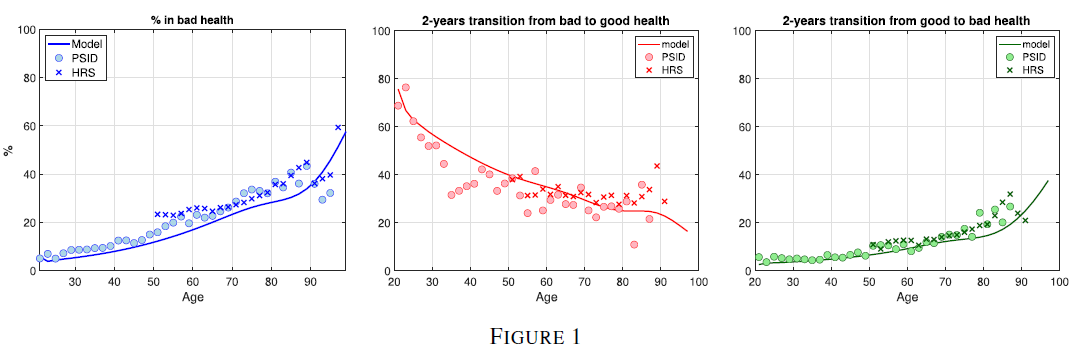
\includegraphics[width=1\linewidth]{figure 1.png}
            \caption{figure 1}
            \label{fig:placeholder}
        \end{figure}
\end{itemize}
}

\frame{\frametitle{Duration matters!}
\begin{itemize}
    \item negative duration dependence
\begin{figure}
    \centering
    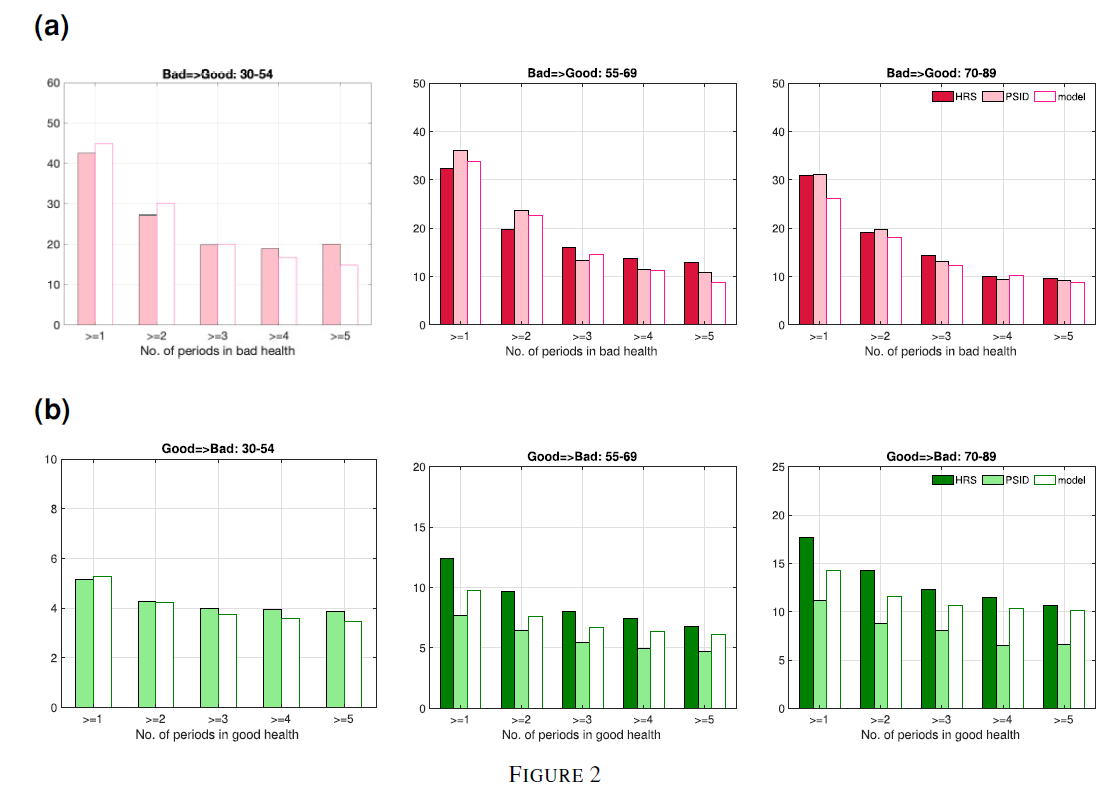
\includegraphics[width=.85\linewidth]{figure 2.png}
    \caption{figure 2}
    \label{fig:placeholder}
\end{figure}
\end{itemize}
}

\frame{\frametitle{Data}
\begin{itemize}
    \item 2 mechanism for negative duration dependence
    \item compounding of health
        \begin{itemize}
        \item modeled by higher order Markov chain. 
        \end{itemize}
    \item ex ante health difference (think genetic, lifestyle)
        \begin{itemize}
        \item different transition probability for different health type
    \item the model try to include both
        \end{itemize}
\end{itemize}
}

\frame{\frametitle{fixed labor productivity and survival probability (estimation)}
\begin{itemize}
    \item Determine how fixed labor productivity related to health.
    \item Look at worker younger than 70, full time (520 hours/year) worker.
    \item $log(inc_{it}) = \sum^{69}_{t=21} \sum_{j = \{G,B\}} d^j_{t}(D^{age}_{it})(D_{h_{it}=j})+\hat{\gamma_{i}} + u_{it}$
    \item Unobserved fixed labour productivity $\hat{\gamma_{i}}$, includes cohort effects in individual fixed productivity.
    \item Regress $\hat{\gamma_{i}}$ with on birth-year dummies to remove cohort effect, denoting the residual of this second regression estimates as $\gamma_{i}$.
    \item composition of fixed labor productivity are different for healthy and unhealthy in both PSID and HRS. 
\end{itemize}
}
\frame{\frametitle{fixed labor productivity}
    \begin{itemize}
        \item composition of fixed labor productivity are different for healthy and unhealthy in both PSID and HRS. 
    \item To model this - allow correlation between fixed labor productivity type and health type
\end{itemize}
\begin{figure}
        \centering
        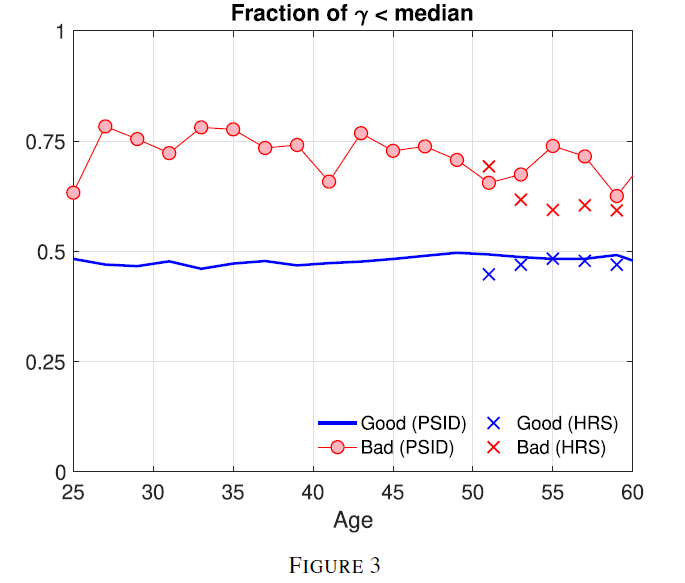
\includegraphics[width=0.35\linewidth]{figure 3.png}
        \caption{figure 3}
        \label{fig:placeholder}
    \end{figure}
}
\frame{\frametitle{constructing unobservable health types}
\begin{itemize}
    \item Use a ordered-logit model to assign/predict health types
    \item $\Pr(\eta \leq \eta_j \mid \mathbf{X}_{t_0}^n) = 
                \begin{cases} 
                \Lambda(b_{\eta j} + \mathbf{B}_\eta \times \mathbf{X}_{t_0}^n) & \text{for } j = \{1, 2\}, \\
                1 & \text{for } j = 3.
                \end{cases}$
    \item X contain fixed productivity tercile dummy {$\gamma_L,\gamma_M,\gamma_H$}, initial health $h_{t0}$, wealth $k_{t0}$, birth-year dummies. 
    \item B is the coefficient for each dummy
    \item $b_{\eta j}$: constant term, $b_{\eta 1} < b_{\eta 2}$
\end{itemize}
}
\section{Health process}
\frame{\frametitle{Health process (the main contribution)}
 \begin{align}
        \begin{split}
            Pr(F_{t+1} \cup P_{t+1}| h_t, \tau_{B}, \eta) = \mathbf{\Lambda}(\sum^{T-1}_{\tau = 1} a^B_{\tau}\mathbbm{1}_{(\tau_B = \tau)}+ a^B_{T}\mathbbm{1}_{(\tau_B \geq T)} \\
            + f^{h_t}_{age}(t) + b_1 + a^{B}_{\eta}D_{\eta})
        \end{split}\\
        \begin{split}
           Pr(F_{t+1} \cup P_{t+1}| G_t, \tau_{G}, \eta) = \mathbf{\Lambda}\Bigg(\sum^{T-1}_{\tau = 1} a^G_{\tau}\mathbbm{1}_{(\tau_{G} = \tau)}+  a^G_{T}\mathbbm{1}_{(\tau_{G} \geq T)} \\
            + f^{G}_{age}(t) + b_2 +a^{G}_{\eta}D_{\eta}\Bigg)
        \end{split}\\
        \begin{split}
            \zeta_{t}(h_{t},\tau_{B}) = \mathbf{\Lambda}\Bigg(\sum^{T-1}_{\tau = 1} a^{\zeta B}_{\tau}\mathbbm{1}_{(\tau_B = \tau)}+ a^{\zeta B}_{T}\mathbbm{1}_{(\tau_B \geq T)}
            + f^{\zeta h_t}_{age}(t)\Bigg)
        \end{split}\\
        \begin{split}
            \zeta_{t}(h_{t},\tau_{G}) = \mathbf{\Lambda}\Bigg(\sum^{T-1}_{\tau = 1} a^{\zeta G}_{\tau}\mathbbm{1}_{(\tau_G = \tau)}+ a^{\zeta G}_{T}\mathbbm{1}_{(\tau_G \geq T)}
            + f^{\zeta h_t}_{age}(t)\Bigg)
        \end{split}
    \end{align}
}

\frame{\frametitle{Transition probabilities of health status}
\begin{itemize}
    \item Combine transition probabilities of health status (equation 1-4) 
    \item health type assignment CDF
    \item estimated survival probabilities
    \item estimated labour productivity fixed effect
    \item Boostrap! B = 10000
    \item maximize log-likelihood
    
    \item$ L(\Theta) = \sum_{i=1}^{N} \log \Bigg( 
        \sum_{j=1}^{3} \Pr(\eta_j \mid \mathbf{X}_{i,t_0}^n) 
        \times \Pr(h_{i,t_0+\tau}, \dots, h_{i,t_0+J} \mid h_{i,t_0}, \dots, h_{i,t_0+\tau-1}, \eta_j) \Bigg)$
    \item where $\Theta$ is the parameters in equations 1,2,3,4, health type assignment function
    \item bootstrapping to get confidence interval
\end{itemize}
}

\frame{\frametitle{Transition probabilities of health status}
\begin{itemize}
    \item Final product of this health dynamic discussion
\begin{figure}
    \centering
    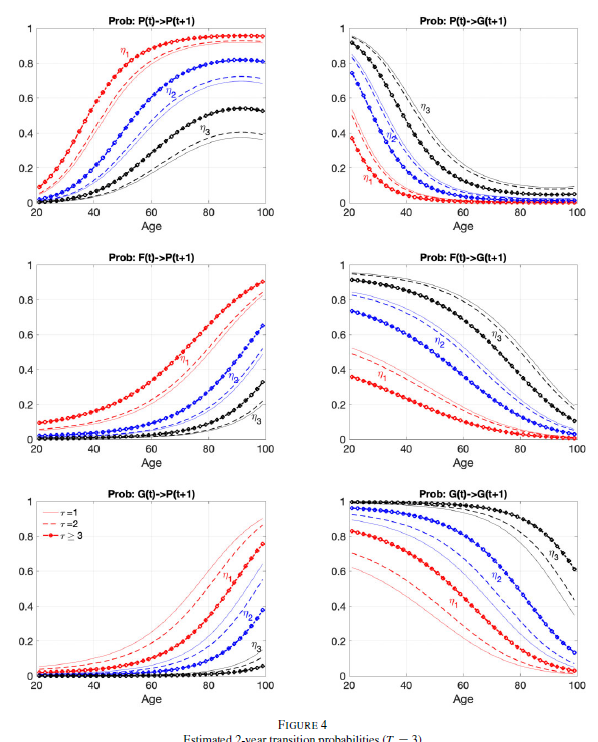
\includegraphics[width=0.5\linewidth]{figure 4.png}
    \caption{estimated 2-year transition prob}
    \label{fig:placeholder}
\end{figure}
\end{itemize}
}

\frame{\frametitle{Transition probabilities of health status}
\begin{itemize}
    \item Final product of this health dynamic discussion
\begin{figure}
    \centering
    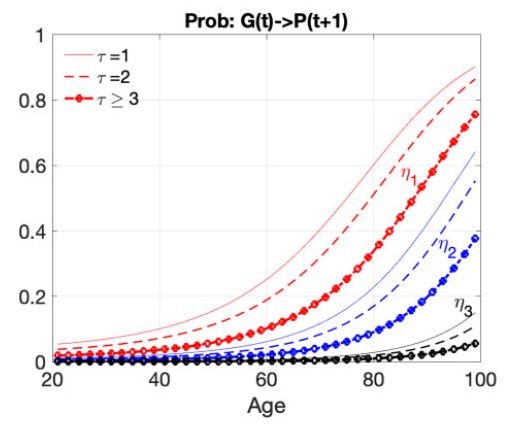
\includegraphics[width=.5\linewidth]{figure 4_sub.png}
    \caption{Prob(P|G)}
    \label{fig:placeholder}
\end{figure}
\end{itemize}
}
\frame{\frametitle{Transition probabilities of health status}
\begin{itemize}
    \item Final product of this health dynamic discussion
    \begin{figure}
        \centering
        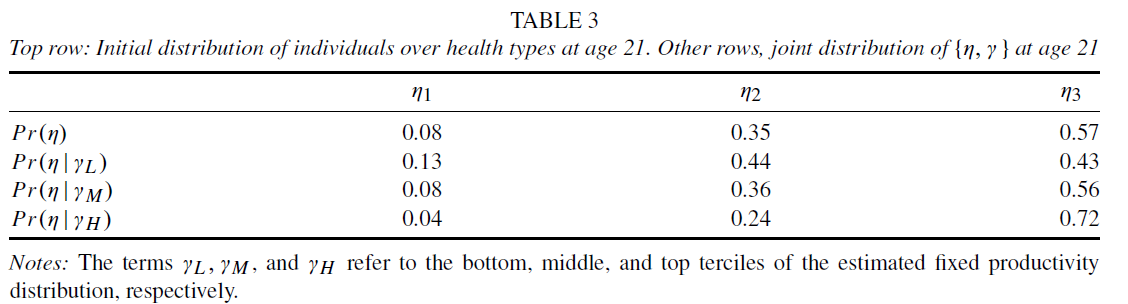
\includegraphics[width=1\linewidth]{table3.png}
        \caption{estimated joint distribution of $\eta, \gamma$}
        \label{fig:placeholder}
    \end{figure}
\end{itemize}
}
\frame{\frametitle{On the existence of health type}
\begin{itemize}
    \item They look at the HRS data
    \item People who are 55-56 years old (high school educated) and alive for the subsequent 10 years
    \item higher \# of unhealthy periods correlate to smoking, higher BMI, lower parent education and longevity at age 55.
    \begin{figure}
        \centering
        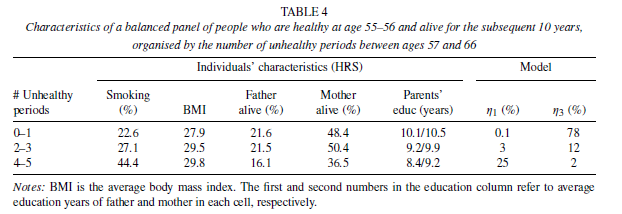
\includegraphics[width=0.75\linewidth]{table 4.png}
        \caption{characteristics at age 55 and future health}
        \label{fig:placeholder}
    \end{figure}
\end{itemize}
}

\frame{\frametitle{On the existence of health type}
\begin{itemize}
    \item also related to genetics (score) for lower educational attainment, higher chance to smoke, higher BMI and lower longevity.
    \begin{figure}
        \centering
        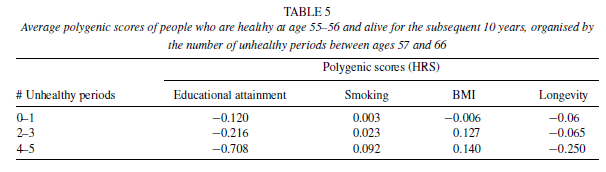
\includegraphics[width=1\linewidth]{table5.png}
        \caption{polygenic score and future health}
        \label{fig:placeholder}
    \end{figure}
\end{itemize}
}

\frame{\frametitle{Endogenous health does not matter}
\begin{itemize}
    \item The health process will break if health can be influenced by decisions.
    \item Medical expenses do not improve health or mortality
    \begin{itemize}
        \item Danesh et al (2024)
                \begin{itemize}
                    \item Free healthcare in Netherland
                    \item high income people still live much longer
                    \item channel: chronic diseases correlated to early age income.
                    \item No significant different in mortality of those with chronic disease across income group. 
                    \item low income group develop chronic disease faster and the difference increases with age.
                    \item Another evidence for ex-ante health difference!
                \end{itemize}
            \end{itemize}
            \end{itemize}
}
\frame{\frametitle{Endogenous health does not matter}
    \item Exercise is overrated
    \begin{itemize}
     \item Include exercise, re-estimate ordered logistics
            \begin{itemize}
                \item existing coefficient: same size and significance 
                \item exercise only plays a preventative role
                \item reduce prob of bad health only if someone is currently healthy and fair
                \item size of coefficient: health type dominate exercise
            \end{itemize}
        \end{itemize}
}

\section{The Life-Cycle Model}
\frame{\frametitle{How health directly affects economic outcomes}
\begin{itemize}

    \item Tow direct mechanisms at work.
    
    \item Incorporate the direct health effects into the structural model.
    
    \item Medical spending.
    
    \item Productivity.

    \item Disutility from work.
    
    \item Access to health insurance.
    
    \item Survival probability.
    
\end{itemize}
}
\frame{\frametitle{How individuals differ Ex-Ante Characteristics}
\begin{itemize}
    \item Fixed labour productivity $\gamma \in \{\gamma_L, \gamma_M, \gamma_H\}$, diecretized into three terciles.
    \item Health type $\eta \in \{\eta_1,\eta_2,\eta_3\}$.
    \item Patience (Discount factor) $\beta \in \{\beta_{low}, \beta_{high}\}, \beta_{low}=0.877 < \beta_{high}=0.992$.
    \item 3x3x2 = 18. 18 Total number of heterogeneity sources in the model!
    \item However, these characteristics can be correlated with each other.
    \item Moment matching $\Pr(\beta_{low} | \eta_{j}) = 
                \begin{cases} 
                0.778 & \text{for } j = 1 \\
                0.794 & \text{for } j = 2 \\
                0.38 & \text{for } j = 3.
                \end{cases}$
    \item Controlling for one's health type $\beta, \gamma$ are independent. 
\end{itemize}
}
\frame{\frametitle{Preferences}
\begin{itemize}
    \item Each period T is two years, retirement set at period $R$, live at most $T$ periods. 
    \item Endowed with 1 unit of time.
    \item Labour supply $l_t$ is indivisible, $l_t \in \{0,1\}$
    \item Fixed cost from working, and working when under poor or fair health, $\phi_W, \phi_F,\phi_P$.
    \item An additional positive term to ensure that individuals value their life (i.e. sick people don't get utility from dying faster)$,\overline{b}$.
    \item $\rho$ is risk aversion and $\overline{n}_t $ is an age-specific household size. 
    \item $u(c_t, l_t, h_t) = \frac{(c_t/\overline{n}_t)^{1-\rho}}{1-\rho} - \phi_W\mathbbm{1}_{\{l_t > 0\}} - \phi_F\mathbbm{1}_{\{h_t=F, l_t > 0\}}-\phi_P\mathbbm{1}_{\{h_t = P,l_t > 0\}} + \overline{b}$
    \item Moment matching $\overline{b} = 7.149$
    \item Set outside $\rho = 3.0, \overline{n}_t1.9-3.2$
\end{itemize}
}
\frame{\frametitle{Bequests}
\begin{itemize}
    \item $v(k) = \theta_{Beq}\frac{(k+k_{Beq})^{1-\rho}}{1-\rho}$
    \item De Nardi (2004).
    \item We have seen this Bequest model many times, $k_{Beq}$ determines to what extent bequest are a luxury good, and $\theta_{Beq}$ determines the strength of the bequest motive. 
    \item Homogenous bequests motives, however this will be affected by agents' ex-ante differences in characteristics. \
    \item Moment matching $\theta_{Beq} = 1,905, k_{Beq} =182,707
    $
\end{itemize}
}
\frame{\frametitle{Labour Productivity process}
\begin{itemize}
    \item Labour income $z_{t}^{h} l_{t}$
    \item Labour productivity $z_{t}^{h} = \lambda_{t}^{h}\Upsilon_{t} = \lambda_{t}^{h}\exp(\upsilon_{t})\exp(\gamma)$,
    \item $\upsilon_t = \rho_{\upsilon}\upsilon_{t-1} + \varepsilon_{t} ; \varepsilon_t \sim N(0, \sigma^2_{\varepsilon}=0.0198), \rho_{\upsilon} = 0.9472 $
    \item $\gamma \sim N(0, \sigma^2_{\gamma} = 0.051 )$. 
    \item If you ignore the fixed productivity $\gamma$ component inside the idiosyncratic competent $\Upsilon_{t}$ and take the log of the labour productivity, this is how we whack TFP using an AR(1) process to generate a real business cycle in DSGE.
    \item $\lambda_{t}^{h}$ is deterministic function of age and current health
\end{itemize}
}

\frame{\frametitle{Medical expenses and health insurance}
\begin{itemize}
    \item At the beginning Medical expense shock $x^{h}_{t}$ realizes. $x^{h}_{t}$ follows the distribution of medical shocks $\mathcal{G}_t(x_{t}^{h}|h_t)$.  
    %\item Working-age people can be uninsured or covered by different types of private insuranc. 
    \item Four types of health insurance: uninsured, individual insurance, employer-sponsored health insurance(ESHI), and Medicare. $i_{H} \in \{0,1,2,3\}$.
    \item $cvg(x_{t}^{h}, i_{H})$ as the fraction of medical expenses covered by insurance.
    \item May purchase individual insurance at market price \\  $p_{I}(h_t,t) = \xi EM_t(h_t,t) + \varphi ^h$. $\varphi$ increases as health status worsen - insurance denial, higher search cost (100 or 2100). 
    \item $\xi = 1.07$
    \item $P_{MCR} = 1,055$
\end{itemize}
}

\frame{\frametitle{Taxation and social transfers}
\begin{itemize}
    \item Medicare tax $\tau_{MCR}$, Social Security tax $\tau_{ss}$, consumption tax $\tau_{c}$ and tax on capital income $\tau_{k}$.
    \item Progressive labour income tax $\mathcal{T}(y) = y - a_{\tau 0} y ^{1-a_{\tau 1}}$, Heathcote et al. (2020)
    \item Public safety-net program, $T^{SI}(\overline{c})=  max\{0, (1+\tau_{c})\overline{c} + Tax + P^{h}_{t} + x^{h}_{t}(1-cvg(x^{h}_{t}, i_{H})) - k_{t}(1+(1-\tau_{k})r) - z_{t}^{h}l_{t}\}$.
    \item Social Security: $ss(h_{R-1}, \upsilon_{R-1}, \gamma, \eta, \beta)$.
    \item Moment matching $\overline{c} = 3,505 $
    \item Set outside $a_{\tau 0} = 0.941, a_{\tau 1}=0.158, \tau_{k} = 0.05, \tau_{c}= 0.36$
\end{itemize}
}

\frame{\frametitle{Timing of the models}
\begin{itemize} 
    \item State variables are: $k_t, h_t \in \{G,F,P\}$, $ \tau\in\{1,2,3\}, \upsilon_t, g_t \in \{0,1\},  t\in \{1,2,...,R-1\}, \gamma \in \{\gamma_L, \gamma_M, \gamma_H\}$, $\eta \in \{\eta_1,\eta_2,\eta_3\}, \beta \in \{\beta_{low}, \beta_{high}\}$. Based on this information, an individual decides labour supply $l_t$, and insurance choice $i_H$.
    \item At the beginning of the period, individuals learn their productivity, health and ESHI offer status. At the end of each period, $x_h^t$ shock is realized, after paying the out-of-pocket medical expenses individual then choose $c_t$ and $k_{t+1}$
    \item control variables for working-age individual are: $l_t, i_H, c_t, k_{t+1}$
    \item control variables for retirees are: $c_t, k_{t+1}$
    \item Denote $\mathbb{S}_{t} = [k_t, h_t, \tau, \upsilon_t, g_t, \gamma, \eta, \beta]$
\end{itemize}
}

\frame{\frametitle{Optimization problem}
\begin{itemize}
    \item Now let's add everything together.
    \item For working-age individuals $(t < R)$
    \begin{align}
        V_{t}(\mathbb{S}_{t}) &= \max_{l_{t}, i_{H}} \sum_{x_{t}^{h}}\mathcal{G}_t(x_{t}^{h}|h_t)W_t(\mathbb{S}_{t}; l_t, i_{H}, x_{t}^{h})
    \end{align} 
    \item where we have interim value function 
    \begin{align}
    \begin{split}
      W_t(\mathbb{S}_{t}; l_t, i_{H}, x_{t}^{h}) &= \max_{c_{t}, k_{t+1}} \{u(c_t, l_t, h_t) + \beta[\zeta_{t}^{h}E_{t}(V_{t+1}(\mathbb{S}_{t+1})) \\
        &+ (1-\zeta_{t}^{h})\theta_{Beq}\frac{(k+k_{Beq})^{1-\rho}}{1-\rho}]\}  
    \end{split}
    \end{align} \end{itemize}
}

\frame{\frametitle{Optimization problem}
\begin{itemize}
    \item subject to
    \begin{align}
    \begin{split}
        k_{t}(1+(1-\tau_{k})r) + z_{t}^{h} l_{t} - x^{h}_{t}(1-cvg(x^{h}_{t}, i_{H})) \\
        - P^{h}_{t} - Tax + T^{SI}(\overline{c}) = (1 -\tau_{c})c_{t} + k_{t+1} \\
    \end{split} \\
    \begin{split}
        T^{SI}(\overline{c}) =  max\{0, (1+\tau_{c})\overline{c} + Tax + P^{h}_{t} + \\
        x^{h}_{t}(1-cvg(x^{h}_{t}, i_{H})) - k_{t}(1+(1-\tau_{k})r) - z_{t}^{h}l_{t}\}\\
    \end{split}\\
    \begin{split}
        Tax = \mathcal{T}(z_{t}^{h}l_{t}) + \tau_{MCR}z_{t}^{h}l_{t} + \tau_{ss}\min\{z_{t}^{h}l_{t}, \overline{y}_{ss}\}
    \end{split}
    \end{align}
    \item Insurance premium: $P_{t}^{h} =$\begin{cases} 
      0 & i_{H} \in \{0,2\}\\
      p_{I}(h_t,t) & i_{H} \in \{1\}\\
   \end{cases}
\end{itemize}
}

\frame{\frametitle{Optimization problem}
\begin{itemize}
    \item For retirees $(t \geq R)$
    \begin{align}
        V_{t}(\mathbb{S}_{t}^{R}) &= \max_{l_{t}, i_{H}} \sum_{x_{t}^{h}}\mathcal{G}_t(x_{t}^{h}|h_t)W_t(\mathbb{S}_{t}^{R}; x_{t}^{h})
    \end{align} 
    \item where we have interim value function 
    \begin{align}
    \begin{split}
      W_t(\mathbb{S}_{t}^{R}; x_{t}^{h}) &= \max_{c_{t}, k_{t+1}} \{u(c_t, 0, h_t) + \beta[\zeta_{t}^{h}E_{t}(V_{t+1}(\mathbb{S}_{t+1}^{R})) \\
        &+ (1-\zeta_{t}^{h})\theta_{Beq}\frac{(k+k_{Beq})^{1-\rho}}{1-\rho}]\}  
    \end{split}
    \end{align} \end{itemize}
}

\frame{\frametitle{Optimization problem}
\begin{itemize}
    \item subject to
    \begin{align}
    \begin{split}
        k_{t}(1+(1-\tau_{k})r) + ss - x^{h}_{t}(1-cvg(x^{h}_{t}, 3)) \\
        - P_{MCR} - \mathcal{T}(ss) + T^{SI}(\overline{c}) = (1 -\tau_{c})c_{t} + k_{t+1} \\
    \end{split} \\
    \begin{split}
        T^{SI}(\overline{c}) =  max\{0, (1+\tau_{c})\overline{c} + \mathcal{T}(ss) + P_{MCR} + \\
        x^{h}_{t}(1-cvg(x^{h}_{t}, 3)) - k_{t}(1+(1-\tau_{k})r) - ss\}\\
    \end{split}
    \end{align}
\end{itemize}
}


\section{Results}

\frame{\frametitle{Results}
\begin{itemize}
    \item Compositional differences and wealth-health gradient 
    \item monetary losses
    \item welfare losses
\end{itemize}
}

\frame{\frametitle{Compositional differences and wealth-health gradient }
\begin{itemize}
    \item Calibration result: time preference and health type is correlated
    \begin{figure}
        \centering
        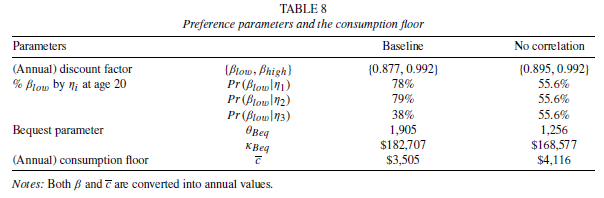
\includegraphics[width=1\linewidth]{table 8.png}
        \caption{second stage estimated parameter}
        \label{fig:placeholder}
    \end{figure}
\end{itemize}
}
\frame{\frametitle{Results}
\begin{itemize}
    \item Compositional differences and wealth-health gradient 
    \item No-correlation model can not replicate wealth-health gradient
    \begin{figure}
        \centering
        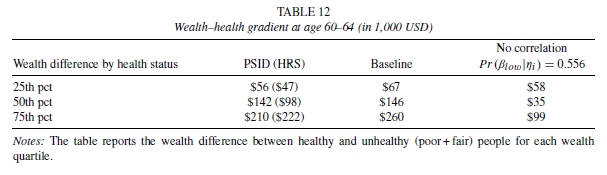
\includegraphics[width=1\linewidth]{table 12.png}
        \caption{wealth-health gradient near retirement}
        \label{fig:placeholder}
    \end{figure}
    \item we need correlation between ex-ante heterogeneity.
\end{itemize}
}

\frame{\frametitle{monetary losses}
\begin{itemize}
    \item monetary loss to bad health
    \item counterfactual experiment (no bad health realization)
\end{itemize}
    \begin{figure}
        \centering
        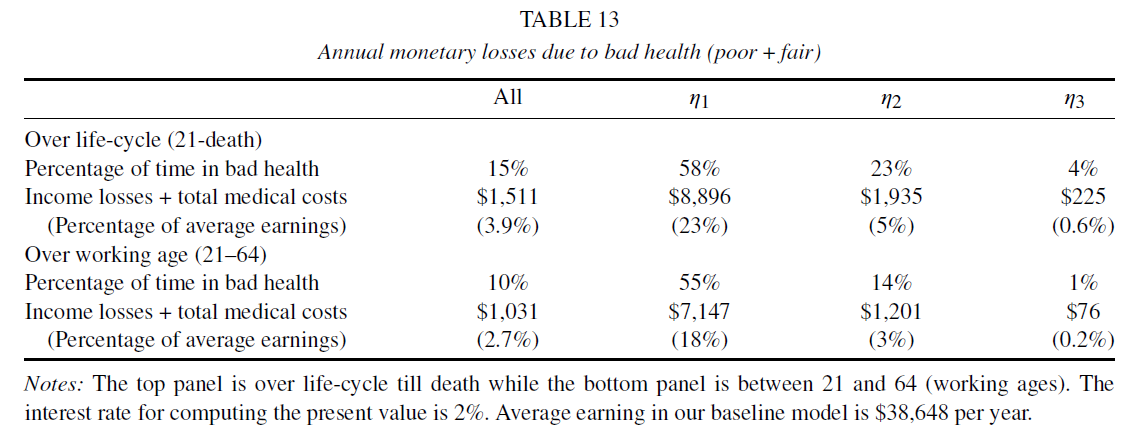
\includegraphics[width=1.0\linewidth]{table13.png}
        \caption{annual monetary losses}
        \label{fig:placeholder}
    \end{figure}
}
\frame{\frametitle{monetary losses}
    \begin{figure}
        \centering
        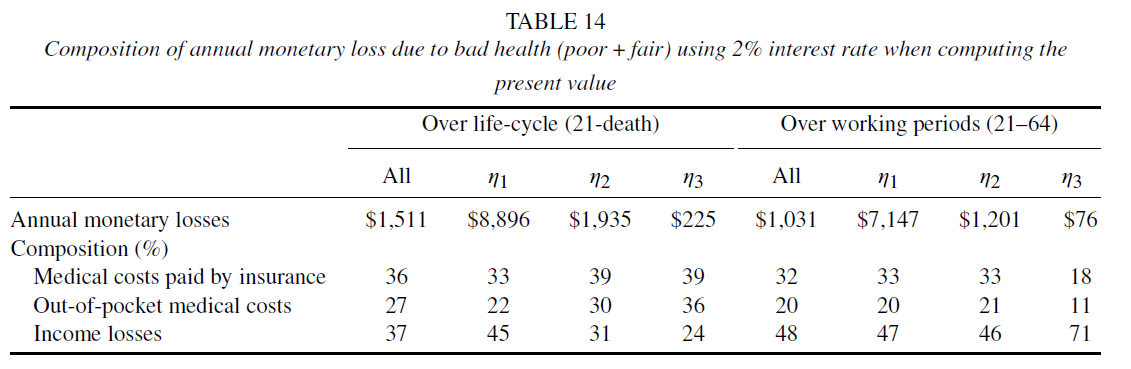
\includegraphics[width=1\linewidth]{table 14.png}
        \caption{Composition of annual monetary losses}
        \label{fig:placeholder}
    \end{figure}
}

\frame{\frametitle{welfare losses}
    \item compensating consumption equivalent (CCE) approach
    \begin{figure}
        \centering
        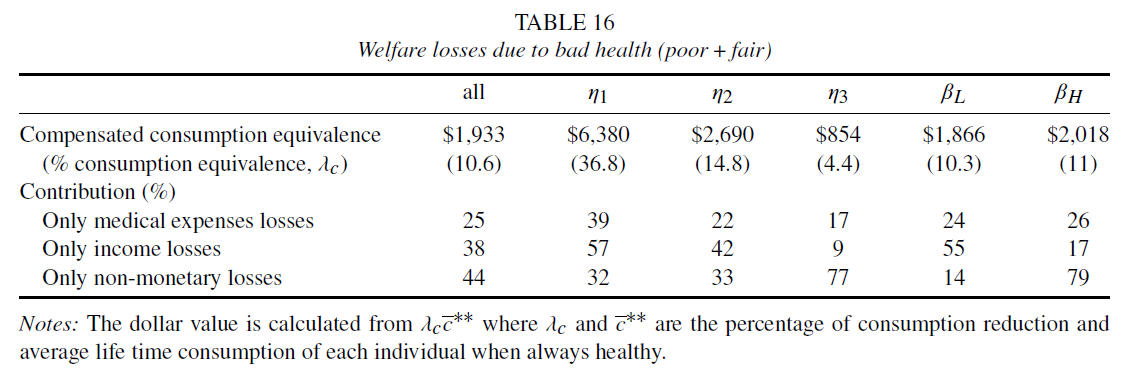
\includegraphics[width=1\linewidth]{table16.png}
        \caption{annual welfare losses due to bad health}
        \label{fig:placeholder}
    \end{figure}
}

\frame{\frametitle{welfare losses}
    \begin{figure}
        \centering
        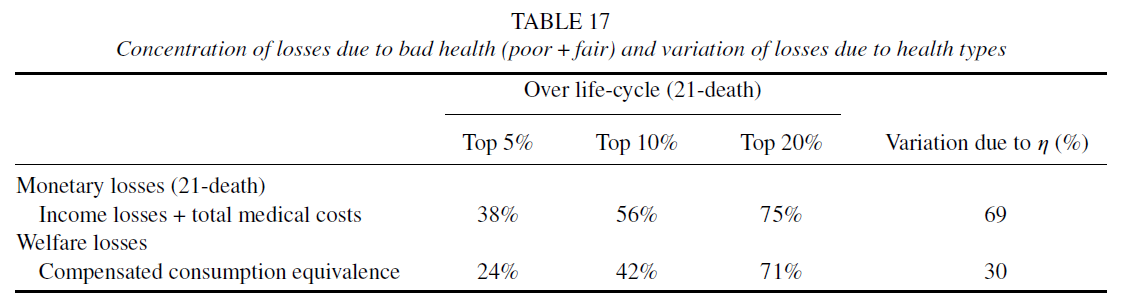
\includegraphics[width=1\linewidth]{table 17.png}
        \caption{Concentration of losses}
        \label{fig:placeholder}
    \end{figure}
}
\end {document}
